\begin{abstract}
Rotary state-space layers such as Mamba-3 apply rotations through cumulative angles, so the gradient with respect to each angle increment is a suffix sum of per-token angular derivatives. In low precision these per-token terms are individually accurate but nearly cancel, and the error of their suffix sum grows roughly as the square root of the sequence length $T$; a more accurate accumulator does not help. We show that, at any cut, the suffix sum equals a Frobenius contraction of the folded trapezoidal state with its adjoint plus a terminal correction that is exactly zero for output-only losses, and we use this identity to evaluate the cross-chunk carry at chunk boundaries. The construction is the rotary analogue of the boundary contractions already used for decay and gate gradients in chunked SSD and gated-linear-attention kernels; omitting the fold or the terminal term gives wrong gradients. We give a deterministic error decomposition, machine-check its algebraic core in Lean~4, and evaluate the method in a pre-registered study of 24 cases and seven methods on one RTX~3080. In the 12 primary cases the angle-gradient error of the boundary method stays at 1.6\% from $T=1023$ to $8192$ (fitted log--log slope $0.00$), whereas BF16 and FP32-intermediate suffix sums grow from 5--6\% to 14--16\% (slope $0.48$--$0.49$). All primary cases meet 2.5\% angle and 1\% timestep targets at a median 4\% captured-backward overhead over BF16, with a median \SpeedGain{} advantage over the fastest qualifying FP32/TF32 baseline under CUDA-graph replay; without graph capture the speed advantage is not consistent. FP32 alternatives remain more accurate at tighter tolerances, and training-level effects are not evaluated.
\end{abstract}
\begin{IEEEkeywords}State-space models, Mamba-3, mixed precision, rounding error, reverse-mode differentiation, rotary embeddings.\end{IEEEkeywords}

\section{Introduction}
\IEEEPARstart{S}{tructured} state-space models (SSMs) process long sequences with chunked algorithms that combine dense intra-chunk products with a short recurrence over chunk states~\cite{ssd}. Mamba-3~\cite{mamba3} adds an exponential-trapezoidal discretization and data-dependent rotations of state coordinate pairs. Because the scalar decay commutes with these rotations, the rotations can be moved onto queries and keys through cumulative angles $\theta_t=\theta_{-1}+\sum_{j\le t}\delta_j$, which keeps the forward pass in matrix-product form. Reverse differentiation then requires, for every increment $\delta_u$, the suffix sum $G_u=\sum_{t\ge u}\partial L/\partial\theta_t$.

This suffix sum is numerically delicate. Rotating every angle of a zero-initial-state sequence by the same amount leaves all outputs unchanged, so the per-token terms nearly cancel: in our emulation the ratio of $\sum_t|g_t|$ to a typical $|G_u|$ grows from about 170 at $T=256$ to more than 5{,}000 at $T=8192$ (Section~\ref{sec:mechanism}). Per-token terms computed from BF16 operands are accurate to about 0.3\%, but their errors do not cancel, and the relative error of $G$ grows roughly as $\sqrt T$. Summing the same terms in FP64 gives the same error, so the problem lies in the terms, not in the accumulator. A public discussion of the Mamba-3 kernels reported exactly this growth (2.8\% at $T=512$ to 11\% at $T=4096$) and suggested computing each suffix sum from the interactions that straddle the cut~\cite{johnsonms}.

This paper turns that suggestion into an exact, implementable chunk-boundary formula and evaluates it. Our contributions are:
\begin{enumerate}
\item A boundary identity (Proposition~\ref{prop:boundary}): for every cut $u$, $G_u$ equals the contraction $\ip{P_u}{X_uJ_i}$ of the \emph{folded} trapezoidal state $X_u$ with its adjoint, plus a terminal correction $\kappa$ from returned final states. $\kappa=0$ exactly for output-only losses, even with nonzero initial states. We show by counterexample that using the unfolded state, or dropping $\kappa$ when final states are differentiated, gives wrong gradients.
\item A chunked realization that keeps local suffix sums only inside a chunk, a metadata policy for $\kappa$ that never consults reference errors, and a deterministic error decomposition that isolates the removed accumulation channel without claiming unconditional length independence.
\item A pre-registered evaluation (24 cases, seven methods, frozen before testing) showing that the boundary error is flat in $T$ while suffix-sum errors grow as $\sqrt T$, together with cost, memory and negative results, including a failed direct-terminal estimator.
\item A Lean~4/Mathlib formalization of the algebraic core of the proof and of the error inequalities, and a reproducibility package with raw data.
\end{enumerate}
We do not claim a new dynamical model or differentiation principle; Section~\ref{sec:related} relates the construction to existing boundary contractions for decays and gates.

\section{Background and related work}\label{sec:related}
\emph{Chunked SSMs and boundary contractions.} In SSD~\cite{ssd}, a cumulative log-decay enters through chunk-local segment sums and a recurrence over chunk states. The reference Triton backward computes the gradient of each chunk-level cumulative decay as a contraction of the stored chunk state with the incoming state gradient (\texttt{ddA = sum(states * dstates) * scale} in the state-passing kernel)~\cite{mambacode}. Chunked gated linear attention~\cite{gla} uses chunk-local cumulative gates, and the backward of the reference implementation~\cite{fla} forms the gate gradient as an intra-chunk suffix sum of $q\odot dq-k\odot dk$ plus a boundary term $\sum h\odot dh$. Our Eq.~\eqref{eq:chunk} has the same structure for rotations: the scaling generator is replaced by the skew generator $J_i$, the state must include the trapezoidal fold, and returned final states contribute $\kappa$. Mamba-3 implementations instead carry cumulative angles across the whole sequence and differentiate them with a global reverse cumsum; we inspected this pattern in the upstream Triton kernel~\cite{mambacode} and in a CUDA kernel~\cite{hf}, and burn-mamba~\cite{burn} contains related cumulative-angle and quaternion-adjoint code.

\emph{Angular precision in Mamba-3.} Pull request~\cite{pr1059} keeps cumulative angles in FP32 and~\cite{pr1070} keeps the raw angle rates in FP32, which reduces phase error in the forward pass. Every variant evaluated here already uses FP32 angles, rates, decays and timesteps; the remaining angle-gradient error comes from the cancellation described above, which Johnsonms~\cite{johnsonms} identified first.

\emph{Symmetry, rotations and precision.} Continuous symmetries constrain gradients~\cite{kunin}; the boundary identity is an instance of this principle for a rotation acting on a suffix of the sequence, made exact by tracking where the symmetry is broken (the cut and the terminal outputs). Rotary position encodings are also sensitive to low-precision phase in attention~\cite{ropebf16}. Reverse-mode differentiation~\cite{ad} and rounding analysis~\cite{higham} are standard; a direct alternative differentiates local rotations without cumulative angles (Appendix~\ref{app:local}), and we use it as an accuracy comparator.

\section{Boundary identity}\label{sec:identity}
For one head, let $S_t\in\mathbb R^{P\times N}$ be a row-coordinate state, $q_t=R(\theta_t)q_t^0$ and $k_t=R(\theta_t)k_t^0$, where $R$ rotates selected coordinate pairs ($R(\theta)=\exp(\theta J)$ in each pair). Define
\begin{align}
X_t&=S_{t-1}+\beta_t v_{t-1}k_{t-1}^{\mathsf T},\label{eq:fold}\\
S_t&=a_tX_t+\gamma_t v_tk_t^{\mathsf T},\quad y_t=S_tq_t,\label{eq:state}
\end{align}
with $a_t=\exp(\mathrm{ADT}_t)$, $\lambda_t=\sigma(\mathrm{Trap}_t)$, $\beta_t=d_t(1-\lambda_t)$ and $\gamma_t=d_t\lambda_t$. Skip and gating terms may depend on angles only through $y_t$. Initial states are independent inputs. The increments are $\delta_{t,i}=\pi d_t\tanh A_{t,i}$.

Let $g_{t,i}=\partial L/\partial\theta_{t,i}$, treating cumulative angles as independent and including any final-angle cotangent at $t=T-1$. Then $G_{u,i}=\partial L/\partial\delta_{u,i}=\sum_{t=u}^{T-1}g_{t,i}$. Let $J_i$ have block $\left[\begin{smallmatrix}0&-1\\1&0\end{smallmatrix}\right]$ in pair $i$ and zero elsewhere.

\begin{proposition}\label{prop:boundary}
With the folded-state adjoint $P_u=\partial L/\partial X_u$,
\begin{align}
G_{u,i}&=B_{u,i}+\kappa_i,\qquad B_{u,i}=\ip{P_u}{X_uJ_i},\label{eq:boundary}\\
\kappa_i&=-\ip{\bar S}{S_{T-1}J_i}+\bar k^{\mathsf T}J_i k_{T-1}+\bar\theta_i,\label{eq:terminal}
\end{align}
where $\bar S,\bar k,\bar\theta$ are cotangents supplied directly to the returned final state, final (rotated) key and final angle. For output-only losses $\kappa=0$, also with nonzero initial states.
\end{proposition}
\begin{IEEEproof}
Shift all suffix angles in pair $i$ by $\varepsilon$. Suffix keys and queries are multiplied by $U=\exp(\varepsilon J_i)$. Equivalently, hold them fixed and replace $X_u$ by $X_uU$: by induction through~\eqref{eq:state}, using $v(Uk)^{\mathsf T}=(vk^{\mathsf T})U^{\mathsf T}$, commutation of $U$ with the scalar decay and $U^{\mathsf T}U=I$, the shifted-angle state equals the perturbed-state solution times $U^{\mathsf T}$, so all suffix outputs agree. Differentiating at $\varepsilon=0$ with $U'(0)=J_i$ gives $B_{u,i}$ from the incoming state. The right factor $U^{\mathsf T}$ on the returned final state, the rotated final key and the returned angle give~\eqref{eq:terminal}; $v$ is not rotated, and the prefix does not depend on $\varepsilon$. Returned angles reduced modulo $2\pi$ are differentiable away from wraps.
\end{IEEEproof}

\begin{remark}
(i)~$P_u$ is the adjoint of the folded state and excludes the readout $y_{u-1}$; pairing $S_{u-1}$ with $\partial L/\partial S_{u-1}$ is wrong. (ii)~For zero initial state, $X_0=0$, so $G_0=\kappa$; for output-only losses the total angular derivative vanishes, which is the global rotation invariance behind the cancellation. (iii)~The chain rule gives $\partial L/\partial A_{u,i}=\pi d_u\operatorname{sech}^2(A_{u,i})G_{u,i}$, and the rotational part of the timestep gradient is $\pi\sum_i\tanh(A_{u,i})G_{u,i}$; other timestep paths are unchanged.
\end{remark}

\emph{Independent checks.} An FP64 sequential autograd implementation agrees with an $O(T^2)$ attention-form reference over 256 cases (16 terminal-cotangent subsets, zero and nonzero initial states, full and partial rotation) and 4{,}800 cuts: maximum normalized identity residual $9.85\times10^{-16}$, all-input gradient disagreement below $10^{-15}$, central finite differences $1.21\times10^{-9}$. A second implementation written only from the equations above reproduces the identity to $1.1\times10^{-15}$ over another 256 cases. In the same code, dropping $\kappa$ when final states are differentiated gives a normalized error of $2.6$, and using the unfolded state with $\partial L/\partial S_{u-1}$ gives $0.18$. A Lean~4 formalization (Appendix~\ref{app:lean}) checks the equivariance induction, the suffix chain rule, the chunk split and the error inequalities below.

\section{Chunked realization and error analysis}\label{sec:realization}
For a chunk ending just before $b<T$, the angular carry from later chunks is replaced by
\begin{equation}
G_{u,i}=\sum_{t=u}^{b-1}g_{t,i}+B_{b,i}+\kappa_i.\label{eq:chunk}
\end{equation}
The final chunk keeps its ordinary local and terminal computation. The contraction $B_b$ reuses the chunk state and adjoint already formed by the chunked backward ($P_b=a_b\,\partial L/\partial S_b$), costs $O(PN)$ per chunk and pair, and is passed to the angle kernel in a small buffer; full per-token states are not stored.

\emph{Terminal policy.} If final states are not returned, all terminal cotangents vanish and we set $\kappa=0$ exactly. If they are returned, we keep the previous estimator $\widehat\kappa=\widehat G_r-\widehat B_r$ at the last chunk start $r$ (``legacy''). The choice uses only API metadata. Direct evaluation of~\eqref{eq:terminal} from computed final states is an ablation: it was not consistently better (Section~\ref{sec:terminal}).

\emph{Error decomposition.} Write $\widehat g_t=g_t+\epsilon_t$, $\widehat B_b=B_b+\Delta B_b$, $\widehat\kappa=\kappa+\Delta\kappa$, and let $\eta_u$ be the arithmetic error of forming~\eqref{eq:chunk}. For each pair,
\begin{equation}
|\widehat G_u-G_u|\le\sum_{t=u}^{b-1}|\epsilon_t|+|\Delta B_b|+|\Delta\kappa|+|\eta_u|.\label{eq:bound}
\end{equation}
Only the explicit local-term sum is bounded by the chunk length; an ordinary suffix sum contains $T-u$ such terms. For inputs $P+E_P$ and $X+E_X$ and contraction rounding $\eta_B$,
\begin{equation}
|\Delta B|\le\norm{P}\norm{E_X}+\norm{X}\norm{E_P}+\norm{E_P}\norm{E_X}+|\eta_B|,\label{eq:inputerror}
\end{equation}
because right multiplication by $J_i$ has Frobenius operator norm $\|J_i\|_2=1$. The contraction has $2P$ products; a sequential non-FMA evaluation satisfies the standard bound $|\eta_B|\le\gamma_{2P}\sum|{\rm products}|$ with $\gamma_n=nu/(1-nu)$~\cite{higham}, which does not transfer unchanged to tensor-core or tree reductions. No independent or zero-mean rounding model is assumed. State, adjoint, phase and terminal errors $E_P$, $E_X$, $\Delta\kappa$ can still grow with $T$, so~\eqref{eq:bound} is not a length-independent guarantee; Section~\ref{sec:results} measures the outcome. Relative errors are ill-conditioned near zero gradients, so such cases are checked with absolute errors.

\section{Experimental setup}\label{sec:setup}
\emph{Implementations.} All variants are modified from the upstream Mamba-3 SISO Triton kernels (snapshot e9594ce)~\cite{mambacode}. Seven methods are compared: (1)~BF16 suffix (upstream angle path with FP32 angles); (2)~FP32 intermediate Q/K gradients; (3)~legacy boundary ($\widehat\kappa$ from the last chunk); (4)~the boundary policy; (5)~FP32 storage with single-pass TF32 dot products; (6)~full FP32 with tf32x3 dot products; and (7)~a direct local-coordinate FP32 adjoint without cumulative angles (Appendix~\ref{app:local}). The Mamba-3-derived kernels evaluate $\tanh$ and $\operatorname{sech}^2$ with the hardware approximation \texttt{tanh.approx.f32}; the references use exact $\tanh$. Configurations were fixed in development: chunk 64 for variants (1)--(4) and (6), chunk 32 for (5) (64 and 128 exceed shared memory on this GPU), local tile 8 for (7) (from 4/8/16), and four-choice backward autotuning (stages 1/2, warps 4/8) for (6). These are tuned implementations, not globally optimal kernels.

\emph{Protocol.} The protocol, including all decision rules below, was frozen and hashed before any test seed was run; the hash is stored in every raw result. Test seeds are 1009, 1013 and 1019 (cotangent seed $+91000$) on four shapes:
\[\begin{array}{rrrrrrr}\text{Shape}&B&T&H&H_q&N&P\\\hline
0&1&1023&8&1&64&64\\1&1&2048&16&4&64&64\\2&2&4097&8&2&64&32\\3&1&8192&16&4&64&32\end{array}\]
The 12 primary cases use the upstream-test-style generator: normalized random Q/K, log-uniform $d\in[10^{-3},10^{-1}]$, decay rates in $[-16,-1]$, BF16 Q/K/V/bias/Trap/Z and FP32 angles/ADT/DT/D. Twelve slow-decay stress cases multiply ADT by $0.01$ with all else matched. Calls use output-only loss, zero initial state, skip and gate. Because $T$ and the head geometry change together, the shapes are not a controlled length sweep.

\emph{Reference and metrics.} References differentiate the mathematical recurrence in FP64 on the exactly represented low-precision inputs with the same BF16 output cotangent, so input quantization is not counted as method error. A hand-derived NumPy adjoint provides large-case references; checkpoint replay is bitwise identical to its uncheckpointed version in 32 checks. We report relative $L_2$ errors of the angle-rate and timestep gradients, the targets of the method (the policy changes no other gradient path); all other input gradients are computed and timed and are validated separately (32 CPU and 18 GPU local-adjoint cases; policy tests at $T\in\{1,63,64,65,2049\}$ with initial/terminal combinations).

\emph{Decision rules.} Primary criteria: median error reduction against the better of BF16 suffix and FP32 intermediates $\ge2$, no case more than 20\% worse than that baseline, $\ge10/12$ cases meeting angle error $\le0.025$ and timestep error $\le0.01$, median speedup over the fastest qualifying non-boundary method $\ge1.5$, and median policy/BF16 overhead $\le1.25$.

\emph{Timing.} One RTX~3080 (10~GB, sm86), Windows~11, Python~3.11.9, PyTorch 2.10.0+cu128, Triton-Windows 3.6.0. One complete backward per method is captured in a CUDA graph on the same stream as the forward~\cite{torch}; nine shuffled rounds replay three backward calls each, and accuracy is checked before and after capture. Compilation is excluded. Ordinary (eager) event and wall times, forward times and precision-promotion costs are recorded separately. GPU clocks were not locked. Timing repeats are not independent scientific cases.

\section{Results}\label{sec:results}
\subsection{Accuracy and length scaling}
All predeclared primary criteria pass (Table~\ref{tab:main}). The policy meets both targets in 12/12 primary cases with median angle error 1.60\% (maximum 1.68\%) and timestep error at most 0.37\%. The median error reduction against the better non-boundary low-precision baseline is \ErrorGain{} (range 3.12--9.14), and no case regresses.

The pooled median depends on the chosen lengths. Fig.~\ref{fig:scaling} and Table~\ref{tab:shape} show the structure behind it: fitting $\log E=\alpha+s\log T$ over the 12 primary cases gives $s=0.49$ for BF16 suffix, $0.48$ for FP32 intermediates and $0.00$ for the policy. The reduction is therefore close to $3.2\sqrt{T/1023}$ (3.16, 4.48, 6.34 and 8.72 for the four shapes). FP32 intermediate Q/K gradients reduce the error by only about 15\%, consistent with the error originating in cancelling local terms rather than in one stored quantity.

Legacy boundary is also flat in $T$ (slope $-0.01$) but larger (median 2.44\%, 7/12 passing). Its error matches the policy when the final chunk has one token ($T=4097$, ratio 1.00) and is 1.5--1.7 times larger when the final chunk has 63--64 tokens, as expected from $\widehat\kappa$ summing the local terms of the last chunk. TF32 storage is more accurate than the policy at these lengths but also grows with $s=0.51$; extrapolating this fit, which we have not tested, it would reach the policy error near $T\approx1.1\times10^4$ and the 2.5\% target near $T\approx2.7\times10^4$. At a 1\% angle target the policy passes 0/12, TF32 9/12, and full FP32 and the local adjoint 12/12.

In the slow-decay stress cases the policy passes 12/12 with median angle error 0.568\% and slope $0.02$, while BF16 suffix grows with slope $0.39$ but still qualifies in 6/12 cases. Boundary evaluation is therefore not always needed at moderate lengths.

\begin{figure*}[t]\centering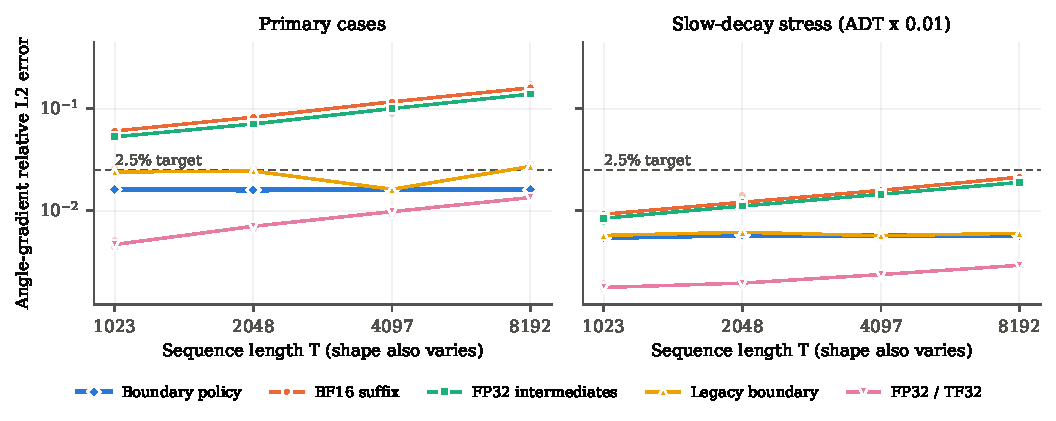
\includegraphics[width=\textwidth]{images/error_vs_length.pdf}
\caption{Angle-gradient relative $L_2$ error versus sequence length (log--log): medians of three seeds with individual seeds as faint points. Fitted slopes (primary/stress): boundary policy $0.00/0.02$, legacy $-0.01/0.01$, BF16 suffix $0.49/0.39$, FP32 intermediates $0.48/0.39$, FP32/TF32 $0.51/0.24$. Head geometry changes with $T$. Full FP32 and the local FP32 adjoint ($<1.3\times10^{-5}$) are omitted for scale.}\label{fig:scaling}\end{figure*}

\begin{table}[t]\caption{Primary cases (12). Pass counts use angle error $\le$1\%/2.5\%/5\% with timestep error $\le$1\%. Time is captured backward, median per-case ratio to BF16 suffix.}\label{tab:main}\centering\small\setlength{\tabcolsep}{3.5pt}
\begin{tabular}{@{}lrrrr@{}}\toprule Method&Median&Max&Pass&Time\\\midrule
\MainTableRows
\bottomrule\end{tabular}\end{table}

\begin{table}[t]\caption{Per-shape medians (primary). Last: tokens in the final chunk. BF16, Policy: angle errors. Red.: error reduction relative to the better of BF16 suffix and FP32 intermediates. Leg./pol.: legacy over policy error. TF32/pol.: TF32 over policy captured backward time.}\label{tab:shape}\centering\small\setlength{\tabcolsep}{3pt}
\begin{tabular}{@{}rrrrrrr@{}}\toprule $T$&Last&BF16&Policy&Red.&Leg./pol.&TF32/pol.\\\midrule
1023&63&0.060&0.0161&3.16&1.53&2.12\\
2048&64&0.083&0.0159&4.48&1.55&1.99\\
4097&1&0.117&0.0161&6.34&1.00&1.39\\
8192&64&0.160&0.0160&8.72&1.70&1.35\\
\bottomrule\end{tabular}\end{table}

\subsection{Mechanism check}\label{sec:mechanism}
To separate the mechanism from the GPU kernels, we recomputed the local terms on the CPU from BF16-rounded operands ($S_t$, $\partial L/\partial S_t$, $q_t$, $k_t$, $v_t$, $\bar y_t$) with FP32 accumulation, for $T=256$ to $8192$ ($P=N=16$, three seeds each). The local terms have relative error 0.28--0.32\%. Their suffix sum has relative error from 1.8\% to 16\% with log--log slope $0.56$; summing the same terms in FP64 changes that error by at most $1.2\times10^{-5}$ in relative terms. The chunked boundary form (chunk 64, $\kappa=0$) gives 1.0--1.4\% with slope $0.015$. These magnitudes are close to the GPU measurements.

\subsection{Cost}
Under CUDA-graph replay the policy costs a median \Overhead{} of BF16 suffix (worst case \WorstOverhead{}). FP32 storage with TF32 dots is the fastest qualifying non-boundary method in every primary case, and the policy is a median \SpeedGain{} faster (range 1.27--2.88). The advantage shrinks with length, from about 2.1 at $T=1023$ to 1.35 at $T=8192$ (Table~\ref{tab:shape}), and these captured times exclude the TF32 path's BF16-to-FP32 promotion (0.12--0.47~ms), which would favor the policy further. In the stress cases, where BF16 often already qualifies, the median advantage over the fastest qualifying method is only 1.07 (range 0.96--1.43).

These speed results depend on graph capture. In ordinary eager execution, recorded in the same runs, TF32 is faster than the policy in 5/12 primary cases and the policy/BF16 ratio varies from 0.66 to 1.74, i.e., launch overhead and noise dominate at these sizes. Without clock locking, the nine captured rounds of one case have a median max/min spread of about 1.3--1.4, and runs of one shape with identical compute differ by up to 1.55 times across seeds and decay settings. We therefore regard the cost result as ``near BF16 cost at moderate accuracy'' on this GPU, not as a general speed claim.

A separate warmed, fresh-process measurement of the complete primitive (forward, backward, promotion and conversion to caller dtypes; seed 1013) gives policy/BF16 peak tensor-memory ratios of 1.0012--1.0017 (policy peaks 12.14--150.27~MiB) and captured speedups over TF32 of 1.37--2.14 (Fig.~\ref{fig:cost}). In this measurement the policy was faster than BF16 suffix in three of four shapes (down to 0.77), although it performs strictly more work; we attribute this to run-to-run variation and do not interpret it. An initial cold measurement that included autotuner allocations is archived and excluded.

\begin{figure*}[t]\centering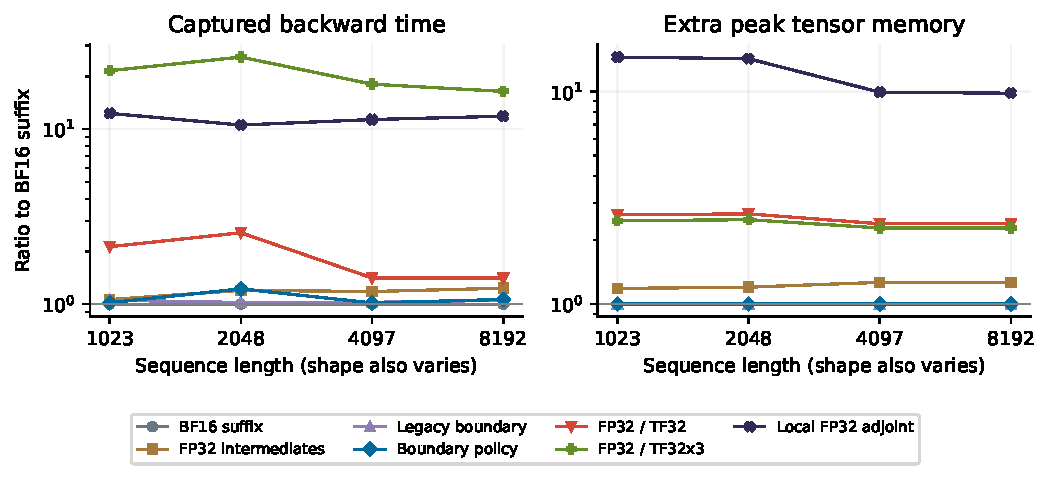
\includegraphics[width=0.82\textwidth]{images/final_cost_memory.pdf}
\caption{Captured backward time (three-seed medians) and warmed peak tensor memory (one fresh process per shape and method), normalized to BF16 suffix. Head geometry changes with $T$.}\label{fig:cost}\end{figure*}

\subsection{Negative result: direct terminal evaluation}\label{sec:terminal}
Before the final study, a separately frozen 36-case study ($T=257$, 2049, 8193, each with a one-token final chunk; initial and terminal objectives varied) tested direct evaluation of~\eqref{eq:terminal} against the legacy estimator. Direct evaluation was worse in 17/36 cases, once by 28\%, and its median improvement on long cases was 1.00013, below the predeclared 1.2 criterion. In the worst case the terminal-correction error was 0.0864 versus 0.0515; contracting the same GPU final states in FP64 still gave 0.0864, so forward state error, not the contraction arithmetic, dominated. This result motivates the metadata policy.

\section{Limitations}\label{sec:limits}
(i)~One GPU model, one operating system and unlocked clocks; no second-machine replication of the GPU study. (ii)~Length and head geometry vary together, and lengths above 8192, where the method's advantage over TF32 should be largest, are untested; the crossover estimates above are extrapolations. (iii)~Inputs come from an upstream-test-style generator, not from trained models, and only one stress multiplier is tested. (iv)~We measure gradient error of a numerical primitive, not training loss, perplexity or downstream accuracy. (v)~The analysis covers scalar decay with commuting pair rotations (SISO); MIMO, variable-length packing and general matrix transitions fall back to the existing path and are not claimed. (vi)~Inherited grouped-query atomic reductions make some K gradients vary across repeats, so bitwise determinism is not claimed. (vii)~The error bound is conditional on state, adjoint and terminal errors, and the Lean development covers the algebraic core rather than an end-to-end proof.

\section{Conclusion}
Boundary evaluation removes the length-growing accumulation channel of rotary angle gradients by replacing the cross-chunk suffix sum with a folded state--adjoint contraction and an exact terminal correction. On the tested shapes the resulting angle-gradient error is flat in $T$ at about 1.6\% for less than 5\% median overhead over BF16, while suffix sums grow as $\sqrt T$. FP32 and local-coordinate adjoints remain the choice for tighter tolerances. Controlled length sweeps beyond 8192 tokens and training-level evaluation are the natural next steps.

\section*{Code and data availability}
Source variants, independent references, the Lean development, raw per-case results with protocol hashes, and scripts that regenerate every number and figure are available at \url{https://github.com/triphopp/rotary-boundary-gradients}.

\section*{Acknowledgment}
AI-based coding and writing assistants were used during implementation, verification and drafting. The author checked all results and takes full responsibility for the content.

\appendices
\section{Local-coordinate adjoint}\label{app:local}
The comparator uses $H_t=S_tR(\theta_t)$ with row rotation $[x_0,x_1]R(\delta)=[x_0\cos\delta+x_1\sin\delta,\,-x_0\sin\delta+x_1\cos\delta]$. For zero initial state,
\begin{align}
F_t&=H_{t-1}+\beta_t v_{t-1}(k_{t-1}^{0})^{\mathsf T}, &
H_t&=a_tF_tR(\delta_t)+\gamma_t v_t(k_t^0)^{\mathsf T},\label{eq:local}
\end{align}
and the readout is $H_tq_t^0$. Let $U_t$ be the adjoint of $H_t$ from future recurrent uses and $\bar y_t$ the output cotangent after the gate, so $P_t=U_t+\bar y_t(q_t^0)^{\mathsf T}$. With $M_t=a_tF_tR(\delta_t)$ and $C_t=\gamma_tP_t+\beta_{t+1}U_t$ ($\beta_T=0$),
\begin{align}
\bar q_t^0&=H_t^{\mathsf T}\bar y_t,\quad\bar k_t^0=C_t^{\mathsf T}v_t,\quad\bar v_t=C_tk_t^0+\text{skip},\nonumber\\
\bar\delta_{t,i}&=\textstyle\sum_p\big(P_{t,p,2i}M_{t,p,2i+1}-P_{t,p,2i+1}M_{t,p,2i}\big),\nonumber\\
U_{t-1}&=a_tP_tR(\delta_t)^{\mathsf T}.\label{eq:localreverse}
\end{align}
With $V_t=v_t(k_t^0)^{\mathsf T}$ and $W_t=a_tv_{t-1}(k_{t-1}^0)^{\mathsf T}R(\delta_t)$: $\overline{\mathrm{ADT}}_t=\ip{P_t}{M_t}$, $\bar d_t|_{\rm direct}=\ip{P_t}{(1-\lambda_t)W_t+\lambda_tV_t}$ and $\overline{\mathrm{Trap}}_t=d_t\lambda_t(1-\lambda_t)\ip{P_t}{V_t-W_t}$. A hand-written implementation of these formulas matches FP64 autograd to $2.7\times10^{-16}$ for every input gradient. The GPU kernel recomputes $M_t$ from the previous state instead of subtracting the current write from $H_t$, includes bias, grouped-query, skip and gate reductions in its timing, stores all states in FP32 and is sequential in time. A later FMA-enabled version passes the same checks and remains slower than TF32 on all four shapes; it is not substituted into the frozen results.

\section{Formal verification}\label{app:lean}
The development (Lean~4.35.0 with Mathlib v4.35.0~\cite{lean4,mathlib}; 22 theorems, no \texttt{sorry}; every theorem depends only on the standard axioms) proves: the transport identities $v(Uk)^{\mathsf T}=(vk^{\mathsf T})U^{\mathsf T}$ and $(SU^{\mathsf T})(Uq)=Sq$; the suffix equivariance induction of Proposition~\ref{prop:boundary} over any commutative ring for any $U$ with $UU^{\mathsf T}=U^{\mathsf T}U=I$, including gated outputs; its specialization to $2\times2$ rotations with $R(\theta+\varepsilon)=R(\varepsilon)R(\theta)$; the chain-rule step from equivariance to the derivative; $\partial(L\circ\mathrm{cum})/\partial\delta_u=\sum_{t\ge u}\partial L/\partial\theta_t$ for any differentiable $L$; Eq.~\eqref{eq:chunk} from the identity at $b$; $\kappa=0$ for output-only losses and $G_0=\kappa$ for zero initial state; inequalities~\eqref{eq:bound} and~\eqref{eq:inputerror} (the latter in any real inner-product space for a linear $J$ with $\|Jx\|\le\|x\|$); and the local-coordinate change of variables~\eqref{eq:local}. The derivative $U'(0)=J$, differentiability of the full recurrence and floating-point rounding models are not formalized.

\section{Reproducibility}
The package records source hashes, upstream Apache-2.0 notices, modified variants and raw results. CPU checks (identity, global and local adjoints, checkpoint replay) run without a GPU and were re-run on a second platform (Linux, Python 3.13, PyTorch 2.15, NumPy 2.5) with all checks passing. Re-running the GPU study requires a compatible GPU; unsupported configurations must be reported rather than dropped. Every number in this paper was recomputed from the raw JSON by a script independent of the analysis pipeline. We report per-shape values instead of cluster-bootstrap intervals, because four shape clusters admit only 16 distinct bootstrap medians.

\begin{thebibliography}{99}
\bibitem{ssd} T. Dao and A. Gu, ``Transformers are SSMs: Generalized models and efficient algorithms through structured state space duality,'' in \emph{Proc. ICML}, 2024. \url{https://arxiv.org/abs/2405.21060}
\bibitem{mamba3} A. Lahoti, K. Y. Li, B. Chen, C. Wang, A. Bick, J. Z. Kolter, T. Dao, and A. Gu, ``Mamba-3: Improved sequence modeling using state space principles,'' arXiv:2603.15569, 2026. \url{https://arxiv.org/abs/2603.15569}
\bibitem{mambacode} State Spaces, ``mamba: Mamba SSM architecture,'' GitHub repository, files \texttt{mamba\_ssm/ops/triton/ssd\_state\_passing.py} and \texttt{mamba\_ssm/ops/triton/mamba3/}, accessed Oct. 2026. \url{https://github.com/state-spaces/mamba}
\bibitem{gla} S. Yang, B. Wang, Y. Shen, R. Panda, and Y. Kim, ``Gated linear attention transformers with hardware-efficient training,'' in \emph{Proc. ICML}, 2024. \url{https://arxiv.org/abs/2312.06635}
\bibitem{fla} fla-org, ``flash-linear-attention,'' GitHub repository, file \texttt{fla/ops/gla/chunk.py}, accessed Oct. 2026. \url{https://github.com/fla-org/flash-linear-attention}
\bibitem{johnsonms} Johnsonms, comment on ``Mamba-3: keep cumulative rotary angles in fp32 in angle\_dt\_fwd,'' state-spaces/mamba pull request 1059, Oct. 2026. \url{https://github.com/state-spaces/mamba/pull/1059}
\bibitem{pr1059} Johnsonms, ``Mamba-3: keep cumulative rotary angles in fp32 in angle\_dt\_fwd,'' state-spaces/mamba pull request 1059, Oct. 2026.
\bibitem{pr1070} Johnsonms, ``Mamba-3 SISO: keep the rotary angle rates in fp32,'' state-spaces/mamba pull request 1070, Oct. 2026. \url{https://github.com/state-spaces/mamba/pull/1070}
\bibitem{hf} Phanerozoic, ``Mamba3 kernel implementation,'' revision 595fa7cfc9b0, accessed Oct. 28, 2026. \url{https://huggingface.co/kernels/phanerozoic/mamba3}
\bibitem{burn} swfsql, ``burn-mamba,'' revision e44d42b7ab12, accessed Oct. 28, 2026. \url{https://github.com/swfsql/burn-mamba}
\bibitem{kunin} D. Kunin, J. Sagastuy-Brena, S. Ganguli, D. L. K. Yamins, and H. Tanaka, ``Neural mechanics: Symmetry and broken conservation laws in deep learning dynamics,'' in \emph{Proc. ICLR}, 2021. \url{https://arxiv.org/abs/2012.04728}
\bibitem{ropebf16} H. Wang, Q. Liu, C. Du, T. Zhu, C. Du, K. Kawaguchi, and T. Pang, ``When precision meets position: BFloat16 breaks down RoPE in long-context training,'' arXiv:2411.13476, 2024. \url{https://arxiv.org/abs/2411.13476}
\bibitem{ad} A. G. Baydin, B. A. Pearlmutter, A. A. Radul, and J. M. Siskind, ``Automatic differentiation in machine learning: A survey,'' \emph{J. Mach. Learn. Res.}, vol. 18, no. 153, pp. 1--43, 2018.
\bibitem{higham} N. J. Higham, \emph{Accuracy and Stability of Numerical Algorithms}, 2nd ed. Philadelphia, PA, USA: SIAM, 2002.
\bibitem{torch} PyTorch contributors, ``CUDA semantics: Stream semantics of backward passes,'' PyTorch 2.10 documentation, accessed Oct. 28, 2026. \url{https://docs.pytorch.org/docs/2.10/notes/cuda.html}
\bibitem{lean4} L. de Moura and S. Ullrich, ``The Lean 4 theorem prover and programming language,'' in \emph{Proc. CADE-28}, 2021, pp. 625--635.
\bibitem{mathlib} The mathlib Community, ``The Lean mathematical library,'' in \emph{Proc. CPP}, 2020, pp. 367--381.
\end{thebibliography}
